\documentclass[tikz,border=5pt]{standalone}
\usepackage{amsmath}
\usepackage{amsfonts}
\usetikzlibrary{shapes.geometric, arrows.meta, positioning, fit, backgrounds, calc}

\begin{document}
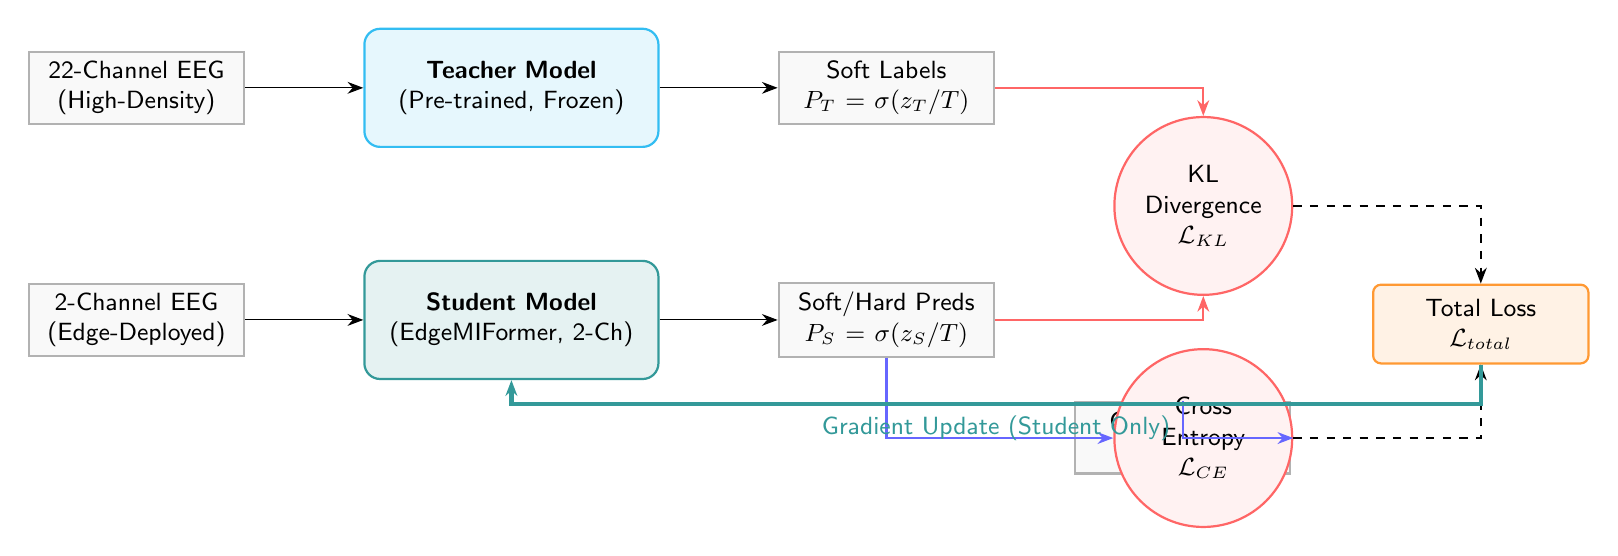
\begin{tikzpicture}[
    font=\sffamily\small,
    >={Stealth[length=2mm, width=1.5mm]},
    model/.style={rectangle, draw=black!60, thick, text width=3.5cm, align=center, rounded corners=2mm, minimum height=1.5cm},
    teacher/.style={model, fill=cyan!10, draw=cyan!80},
    student/.style={model, fill=teal!10, draw=teal!80},
    data/.style={rectangle, draw=gray!60, fill=gray!5, thick, text width=2.5cm, align=center, minimum height=0.8cm},
    loss/.style={circle, draw=red!60, fill=red!5, thick, inner sep=2pt, align=center, minimum size=1cm}
]

% Inputs
\node[data] (in_t) {22-Channel EEG\\(High-Density)};
\node[data, below=2cm of in_t] (in_s) {2-Channel EEG\\(Edge-Deployed)};

% Models
\node[teacher, right=1.5cm of in_t] (teach) {\textbf{Teacher Model}\\(Pre-trained, Frozen)};
\node[student, right=1.5cm of in_s] (stud) {\textbf{Student Model}\\(EdgeMIFormer, 2-Ch)};

% Outputs
\node[data, right=1.5cm of teach] (out_t) {Soft Labels\\$P_{T} = \sigma(z_T / T)$};
\node[data, right=1.5cm of stud] (out_s) {Soft/Hard Preds\\$P_{S} = \sigma(z_S / T)$};

\node[data, right=1cm of out_s, yshift=-1.5cm] (gt) {Ground Truth\\Labels $y$};

% Losses
\node[loss, right=1.5cm of out_t, yshift=-1.5cm, text width=1.8cm] (kl) {KL\\Divergence\\$\mathcal{L}_{KL}$};
\node[loss, right=1.5cm of out_s, yshift=-1.5cm, text width=1.8cm] (ce) {Cross\\Entropy\\$\mathcal{L}_{CE}$};

% Optimizer
\node[rectangle, draw=orange!80, fill=orange!10, thick, rounded corners=1mm, right=1cm of kl, yshift=-1.5cm, minimum height=1cm, text width=2.5cm, align=center] (total) {Total Loss\\$\mathcal{L}_{total}$};

% Arrows Flow
\draw[->] (in_t) -- (teach);
\draw[->] (in_s) -- (stud);
\draw[->] (teach) -- (out_t);
\draw[->] (stud) -- (out_s);

% Loss Connections
\draw[->, thick, red!60] (out_t.east) -| (kl.north);
\draw[->, thick, red!60] (out_s.east) -| (kl.south);

\draw[->, thick, blue!60] (out_s.south) |- (ce.west);
\draw[->, thick, blue!60] (gt.north) |- (ce.east);

\draw[->, thick, dashed] (kl.east) -| (total.north);
\draw[->, thick, dashed] (ce.east) -| (total.south);

\draw[->, ultra thick, teal!80] (total.south) -- ++(0,-0.5) -| (stud.south) node[pos=0.25, below] {Gradient Update (Student Only)};

\end{tikzpicture}
\end{document}
